\chapter{Implementation}
\label{chapter:implementation}

This section outlines the application of data mining process. In this thesis python programming language is used to implement various data augmentation as well as to build deep learning model. Deep learning is implemented using Keras. ``Keras is a high-level neural network API written in Python and is capable of running on top of TensorFlow, CNTK or Theano''-- \citep{chollet2015keras}.  

\section{Business understanding}
As outlined in the motivation section, case company manufactures the portable near-infrared spectrometer. Near-infrared spectroscopy(NIRs) can measure the chemical composition of biological materials by analyzing the diffuse reflectance or transmittance of the samples at several wavelengths from 700 to 2500 nanometers. One of the unique properties of infrared spectrum is that no two organic compounds have the same infrared spectrum \citep{rsc}. Pure compounds can be identified by examination of their spectra provided that a chemist has a copy of the spectrum so any unknown pure compound can be identified by making a comparison \citep{rsc}. This process is straightforward in theory, however in practice due to sample variation, environmental factors and device variations, spectra from two same compounds might not necessarily be identified by making a simple comparison. That is why a machine learning model is needed which takes into consideration several factors and can identify compound based on previously trained data.

NIRs has been widely used in various food commodities especially in the grain, cereal products, and oil-seed processing industries \citep{elmessery2014manufacture}. It is also extensively used in chemical and pharmaceutical industries for classification of raw materials \citep{elmessery2014manufacture}. NIRs technology is gaining popularity for material detection as it is fast, reliable, non-destructive, and relatively cheaper \citep{evans1999near}. Furthermore, there is very minimal sample preparation, or pretreatment and material are preserved after the examination. Therefore NIRs solution provides various advantages over the other types of material sensing solutions.

One of the major hindrances for the application of NIRs has been the size and cost. Conventional spectrometers are relatively big and are also costly. However, the spectrometers produced by the case company are portable and economical. As discussed above, portability adds some complexities, however the advantages over-weight the drawbacks. The portability offers a novel application of NIRs solution in various mass markets, not just limited to traditional agricultural and pharmaceutical industries. 

Overall innovative NIRs solution offered by the case company has significant potential and offers quite many advantages over a traditional sensor. Despite its advantage, there are also several challenges. Traditionally the measurement with the spectrometer is carried out in a controlled environment in a laboratory setting where the environmental variables such as temperature, lights and moisture level can be controlled, enabling consistent measurements. Due to the portable nature of the product, above mentioned environmental variables cannot be controlled. The fluctuation in environmental variables introduces fluctuation in a measurement. The fluctuation of measurement means that the classifier needs to be trained in a diverse sample of data, mimicking the actual use condition. Similarly, samples in the real world come from various sources with a various level of concentration. At present companies try to capture all the environmental as well as sample variation in a laboratory to produce training samples. However, there are several variations, and this takes a considerable amount of time to produce data to train a deep learning model. Similarly, due to regulatory restriction pharmaceutical materials are not readily available, restricting the pool of available samples to train a deep learning model to identify the pharmaceutical material. Furthermore, due to the nature of the manufacturing process, no two scanners are the same. So this means there will be slight variation in a measurement of the same sample from two different scanners. Therefore there is a need for robust model that can take various factors in consideration and correctly classify materials. 

The primary business objective is to produce a robust model that can classify material from the measurement data produced from the portable spectrometer with reasonable accuracy despite all the challenges discussed above. The aim is also to reduce the data acquisition cost and time. To achieve this business goal, data augmentation with deep learning is deemed to be the suitable tool, as data augmentation has the potential to save both time and money in data collection and also improve the generalization ability of the model by increasing the diversity of samples. As mentioned above, there is a precedence of data augmentation being used in a similar situation with a successful result.  

\section{Data understanding}
The primary source of data analyzed in this thesis comes from the NIR spectrometer. A spectrometer analyses a compound by passing near-infrared radiation over a range of different frequencies and measuring the absorption made by each type of bond in a compound. This produces a spectrum, usually a plot of percent transmittance against wave-number. In simple words, transmittance describes how much light passes through a sample unchanged and is measured as a percentage. The image illustrated in figure ~\ref{fig:Spectral data} below illustrates the typical data obtained from spectrometer which is a plot of percent transmittance against wave-number.

\begin{figure}[ht]
	\begin{center}
		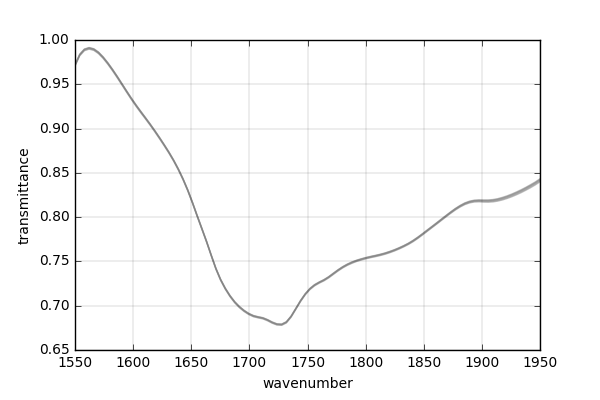
\includegraphics[width=\textwidth]{images/spectral_graph.png}
		\caption{Spectral data}
		\label{fig:Spectral data}
	\end{center}
\end{figure}


As discussed above NIRs is used extensively in pharmaceutical industry to detect raw materials. Incidentally, pharmaceutical raw materials are also among the most heavily regulated materials, so there is limited sample available for training a neural network. As a result, pharmaceutical raw materials are ideal for testing effectiveness of data augmentation. The model built in the thesis will try to detect four different pharmaceutical raw materials. These four different pharmaceutical compounds will be called as variables '0',1','2','3' and '4' respectively. These variables are coded as a categorical variable with label '0','1','2','3' and '4'.

\subsection{Exploratory Analysis}
Pharmaceutical compounds '0', '1','2' and '3' are closely related to each other but are not the same compound. Whereas the compound '4' contains several different compounds that do not belong to any '0','1','2' and '3'. Essentially compound '4' comprise of compounds which  are unknown. The target variables are not 100 percent pure compound. The concentration of the target varies anywhere from 5 to 100 percent. Figure ~\ref{fig:variable concentration} shows the concentration count for all the compound.

\begin{figure}[ht]
	\begin{center}
		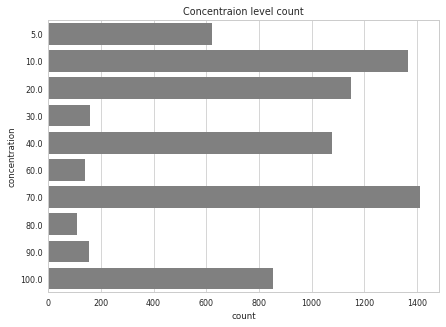
\includegraphics[width=\textwidth]{images/variable_composition.png}
		\caption{Concentration level of compounds}
		\label{fig:variable concentration}
	\end{center}
\end{figure}

As we can see from the figure ~\ref{fig:variable concentration} concentration varies quite a lot. Most compounds have the concentration of 70 percent followed by the 10 percent. Not many compounds have the concentration level of 80 percent. The concentrations of unknown samples are unknown and therefore are not shown in the figure~\ref{fig:variable concentration}. The task of the classifier is to detect the compound regardless of the concentration. Given the spectral data, the classifier has to detect whether there is a presence of target compound or not irrespective of its concentration level. 

The compound '0','1','2' and '3' are hard to acquire, and therefore the data is very imbalanced. Label '4' which represents the samples that do not belong to '0','1','2' and '3' are readily available, and therefore this label is the majority label or class.

\section{Data preparation}

 Spectral data is collected from the spectrometer and stored in a central database. The data does not need extensive data preparation as it is reasonably clean with some exception of missing labels. To prepare the data, samples with missing labels are removed, and the data is transformed using a couple of domain-specific data transformations such as Fourier transformation. Fourier transformation takes a signal and expresses it in terms of the frequencies of the waves that make up that signal. These transformations enable us to compress the data to 50 points from 100 points of spectra.

As discussed earlier, data preparation phase included all the steps undertaken to create a final data-set that is fed to the deep learning model. Consequently, data augmentation is a part of this phase. Above mentioned augmentation techniques, namely data warping, SMOTE, and GANs, will be implemented in the following sub-section.

\subsection{Data augmentation using data warping}
Data warping is one of the simplest and easiest ways to apply data augmentation. In a prominent neural network implementation library Keras, data augmentation for images such as transformation, scaling, rotation and other similar transformations are natively supported. As described earlier, data warping creates new data primarily using a transformation that rotates, shifts or adds distortion which still preserves the label. This type of augmentation for image data is quite straightforward as these types of transformations preserve the image label. For example, rotated image data of a cat still retains its label as cat image upside down is still a cat image. However, for spectral data, augmenting the data by rotation no longer preserves the label. In this sense augmenting data using the data warping technique is highly domain specific and requires a thorough understanding of data at hand.

For spectral data, the appropriate augmentation was to add a small amount of randomly distributed slope so that the points are slightly shifted up or down from the original data. By adding a small amount of slope, we assumed that it could mimic the variation caused by measuring the same sample under different conditions such as humidity, temperature and sample concentration. The figure below illustrates the augmentation on the spectral data along with the similar augmentation on image data. The simple algorithm used to augment data is presented in appendix~\ref{chapter:first-appendix}.

\begin{figure}[ht]
	\begin{center}
		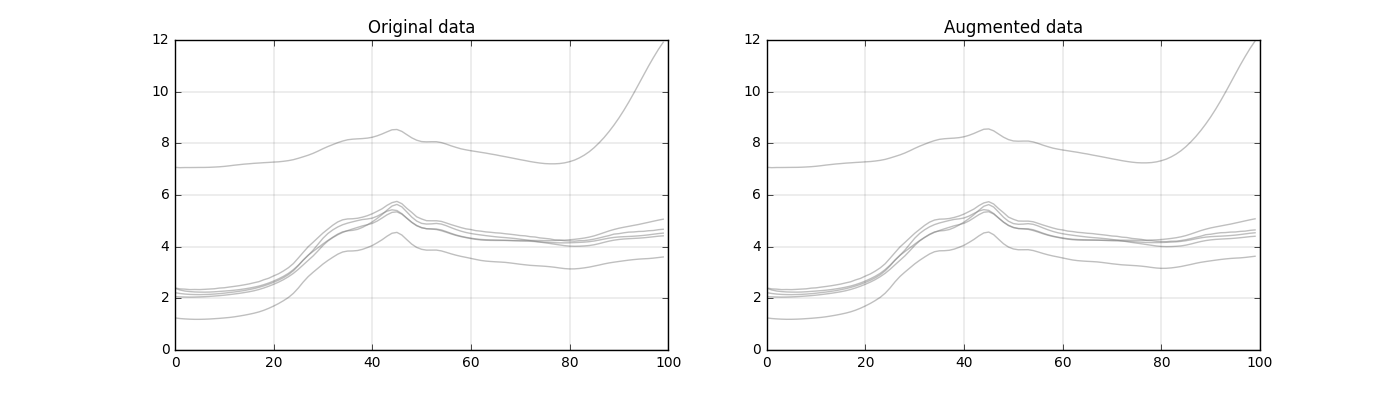
\includegraphics[width=\textwidth]{images/simple_augment.png}
		\caption{Augmentation using data warping}
		\label{fig:simple augmentation}
	\end{center}
\end{figure}


The random points added to the original point is minimal, therefore augmented data is not easily differentiable from the original. However, on close observation, we can observe that augmented data have points slightly up or down compared to the original figure. This type of data augmentation is akin to distorting the image by adding random noise. Depending upon the augmentation the value of noise can be increased or decreased by adjusting the parameters from where the random noise is generated. 

\subsection{Data augmentation using SMOTE} 
SMOTE was conceived to better handle the imbalance data-sets by oversampling the minority class. What SMOTE does is it leaves the majority class intact, in this case unknown samples, and it creates synthetic samples for all other minority classes so that all the class labels are represented equally in the final data set. The details of how SMOTE is implemented is already discussed in the theoretical review section. The augmentation using SMOTE was implemented via python module called 'imblearn' \citep{JMLR:v18:16-365}. This implementation is displayed in appendix~\ref{chapter:second-appendix}. Figure ~\ref{fig:SMOTE augmentation} shows the generated synthetic samples from SMOTE. 


\begin{figure}[ht]
	\begin{center}
		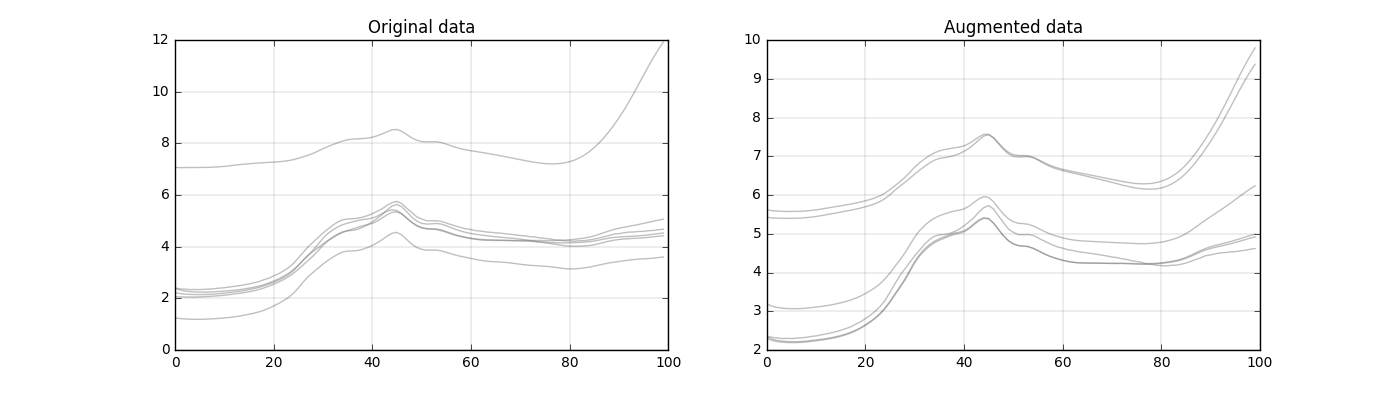
\includegraphics[width=\textwidth]{images/smote_augment.png}
		\caption{Augmentation using data warping}
		\label{fig:SMOTE augmentation}
	\end{center}
\end{figure}

In the figure~\ref{fig:SMOTE augmentation} we can see that augmented data have a bit more variation than the augmented data through data warping. The new generated spectral data is just an interpolation of new data between existing data. As we can observe from the figure~\ref{fig:SMOTE augmentation} original y value is within the range of 1 to 12, and the augmented data y value is also within that same range. One can argue that this behavior is ideal because in a field setting the spectrometer measurement can fluctuate within the range of training samples.  

The overall idea of augmentation in SMOTE is quite similar to data warping. The augmented data is merely shifted up or down. However, in data warping the data was created simply by adding random points to one spectral data. Here the data is interpolated between a spectral data and its k-nearest neighbor. This technique increases the variation of the sample compared to data warping.   
 
\subsection{Data augmentation using GANs}
To implement the GANs laid out in the literature review we make two deep learning models: one generator and another discriminator. Then we stack together the two models and start a model training process. The architecture of the GANs model is illustrated in the figure below.

\begin{figure}[ht]
	\begin{center}
		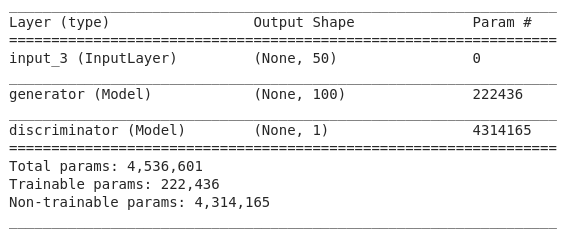
\includegraphics[width=\textwidth]{images/GAN_architecture.png}
		\caption{Augmentation using data warping}
		\label{fig:GAN architecture}
	\end{center}
\end{figure}

Here the generator model turns a vector that is randomly sampled from normal distribution into a data mimicking the actual data generated from the sensor. One common problem with GANs is sometimes generator gets stuck with generating data that is just noise. A possible solution is to use a dropout layer on both the discriminator and the generator. Here the discriminator model takes as input a data that is generated or actual and classifies it into one of two classes: ``generated data''  or  ``real data''.

The figure~\ref{fig:GAN architecture} shows a GANs network architecture in Keras interface. In GANs architecture two models, discriminator and generator, are chained together into GANs network. When trained, the model will move the generator in a direction that improves its ability to fool the discriminator. Generator and discriminator are just two neural networks.

The first step of the training process is to draw random points from the normal distribution, and then generate a data from those random points. The second step is to mix the generated data with actual data, then label it either ``real'' or ``generated'' and feed it into the discriminator. The third step is to draw new random points from a normal distribution and train GANs using these random vectors, which are all labelled as ``real''. This third step effectively updates the weights of the generator to move them toward getting the discriminator to predict ``real'' for generated data \citep{chollet2017deep}. The figure~\ref{fig:GANs augmentation} shows the generated images from the GANs. From the figure~\ref{fig:GANs augmentation} we can see that augmentation from GANs is unlike any other before. The other augmentation strategies closely replicated the actual shape of original data, whereas generated data from GANs do not have smooth slopes like original data. The full implementation using python and Keras is illustrated in appendix~\ref{chapter:third-appendix}.


\begin{figure}[ht]
	\begin{center}
		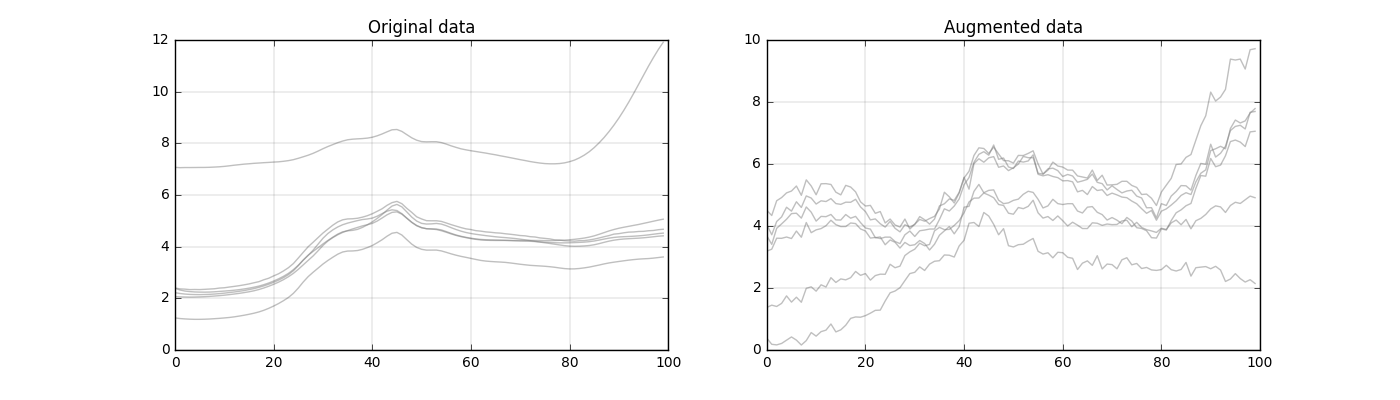
\includegraphics[width=\textwidth]{images/gan_augment.png}
		\caption{Augmentation using data warping}
		\label{fig:GANs augmentation}
	\end{center}
\end{figure}

\section{Modeling}
In this phase, we build deep learning models using data prepared through different augmentation methods. A neural network was chosen primarily because of its ability to handle high dimensional data, the requirement of little feature engineering and the availability of open source libraries that can leverage graphical processor for a speedy result. There are various types of neural networks, and in this thesis, we will be working with the kind of network known as the convolutional neural network.

Convolutional neural network was chosen primarily because unlike the typical dense layers, convolution layers learn local patterns in their input feature space whereas dense layers learn global patterns \citep{chollet2017deep}. Furthermore, convolution net can learn the spatial hierarchies of patterns. These critical characteristics of convolution net makes it translation invariant, meaning that the convolution net can recognize the patterns, no matter where they are. \citep{chollet2017deep}. For example, convolution network is quite successful in image classification because it can detect the local patterns along with its spatial hierarchies such as eye, nose and mouth, no matter where they are located in the image. Since we are treating the data obtained from spectrometer as a fingerprint of the particular chemical compound, identifying local patterns and hierarchies in spectral data can help in accurately classifying one fingerprint from another. The figure~\ref{fig:Convolution model} illustrates the architecture of the convolution neural network used for modeling. 

The model was trained for 30 epochs in mini-batches of 2000 samples. Epoch means merely the number of iteration over all the samples in training data, whereas batch is the number of training data that is used to update the weights. We do not pass the entire data set into the neural network at once but instead divide the data into a number of small batches. On completion of every batch, the loss is computed, and weights of networks get updated.


\begin{figure}[ht]
	\begin{center}
		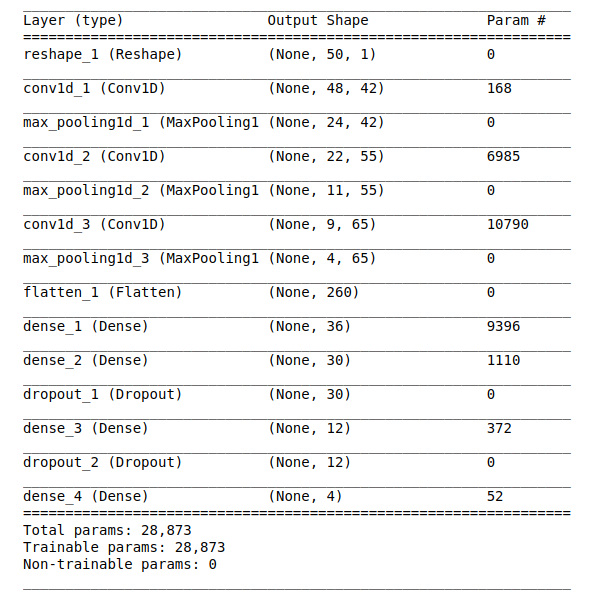
\includegraphics[width=\textwidth]{images/Convolution_model.png}
		\caption{Model Architecture}
		\label{fig:Convolution model}
	\end{center}
\end{figure}

Picking the right network architecture is more of an art than a science-- \citep{chollet2017deep}. Having said that, there are some best practices and generally accepted conventions. The architecture of network proposed in the thesis is based on the best practices and generally agreed principles. For instance, categorical cross-entropy is used as the objective function of the model, as it is generally used for multi-class classification problems. Similarly, convolutional layers are followed by a max-pooling layer which is also a common practice in designing convolutional network. 

In summary, in the implementation chapter we have implemented various data augmentation techniques and generated artificial spectral data. Similarly we have also implemented convolutional neural network to classify pharmaceutical material. 